% This example is meant to be compiled with lualatex or xelatex
% The theme itself also supports pdflatex
\PassOptionsToPackage{unicode}{hyperref}
\documentclass[aspectratio=1610, 9pt]{beamer}

% Load packages you need here
\usepackage{polyglossia}
\setmainlanguage{english}

\usepackage{csquotes}
    

\usepackage{amsmath}
\usepackage{amssymb}
\usepackage{mathtools}
\usepackage{siunitx}
\usepackage{booktabs}

\usepackage{pgfpages}
\setbeameroption{show notes on second screen}

\usepackage[
  style=numeric,
  sorting=none,
  backend=biber,
]{biblatex}
\addbibresource{references.bib}

\usepackage{hyperref}
\usepackage{bookmark}

\usepackage{xfrac}
\usepackage{tikz}
\usetikzlibrary{
  overlay-beamer-styles,
  calc,
  tikzmark,
  decorations.pathreplacing,
}

% load the theme after all packages

\usetheme[
  showtotalframes, % show total number of frames in the footline
]{tudo}

% Put settings here, like
\unimathsetup{
  math-style=ISO,
  bold-style=ISO,
  nabla=upright,
  partial=upright,
  mathrm=sym,
}

\newcommand{\roundpic}[6][]{
  \node [circle, draw, color=tugreen, minimum width = #2,
    path picture = {
      \node [#1] at (path picture bounding box.center) {
        \includegraphics[width=#3]{#4}};
    }] at (#5,#6) {};}


\title{High-level Event Reconstruction for the LST-1 Prototype of the Cherenkov Telescope Array}
\author[L.~Beiske]{Lukas Beiske}
\institute[E5b]{E5b Astroparticle Physics \\  Department of Physics - TU Dortmund}
\titlegraphic{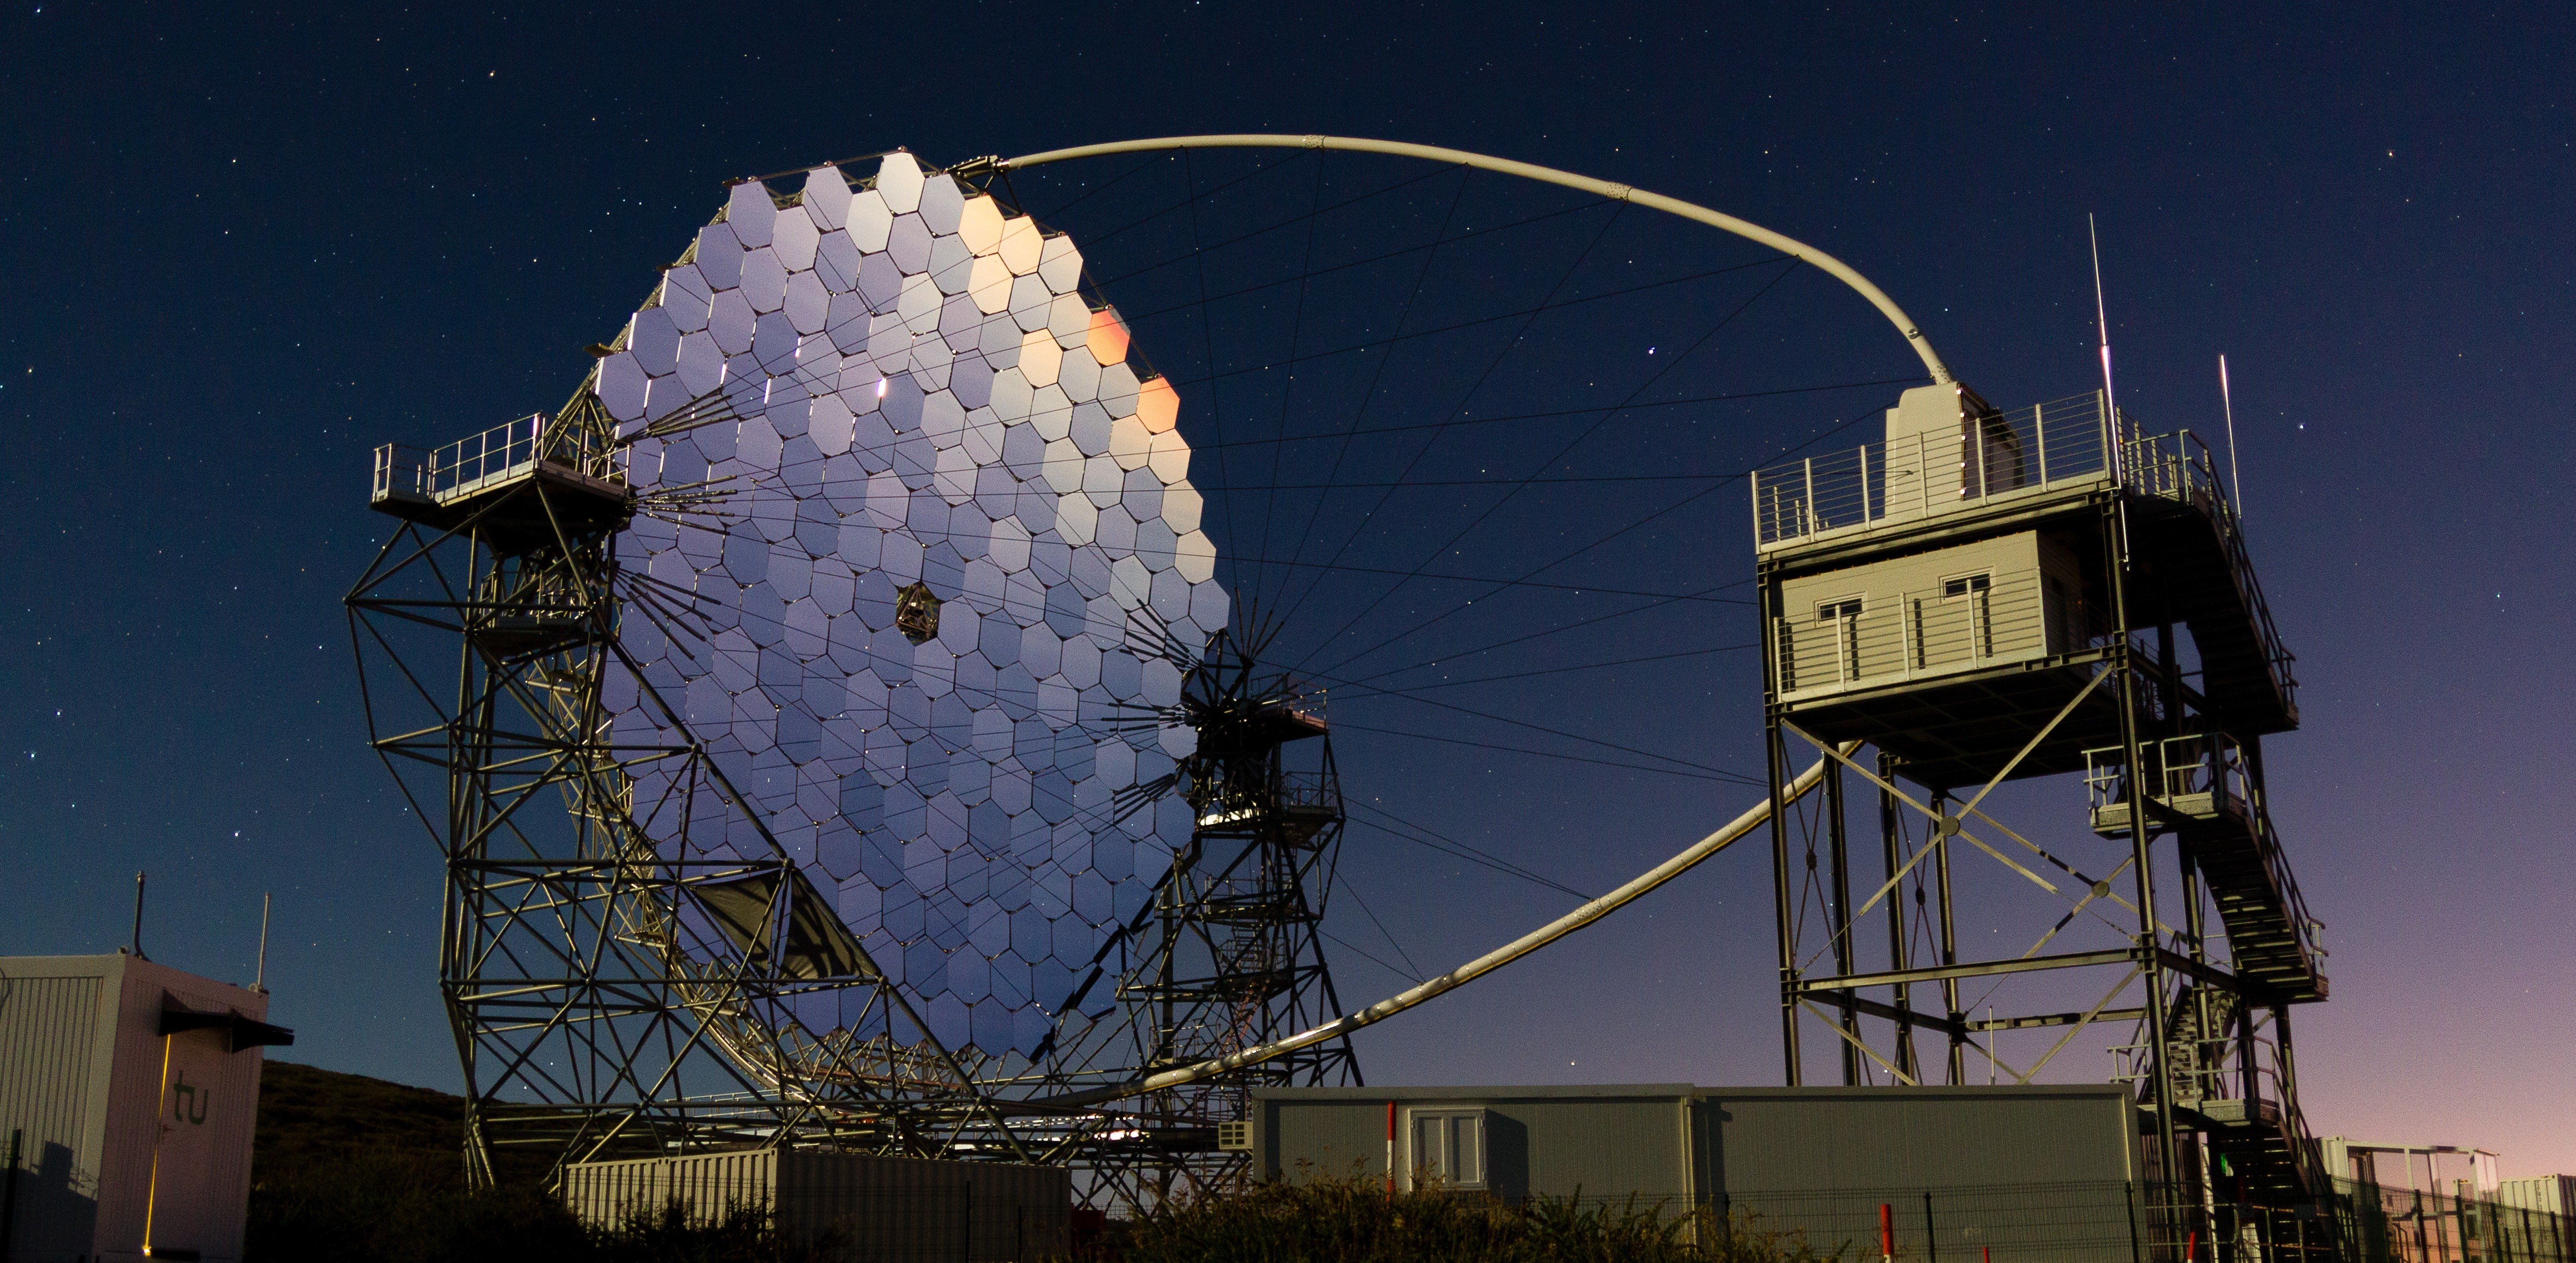
\includegraphics[width=0.5\textwidth]{images/LST_2.jpg}}


\begin{document}

\maketitle

\begin{frame}{Overview}
  \tableofcontents
\end{frame}

\section{Introduction}
\chapter{Gamma-Ray Astronomy}
In astronomy observations can be conducted using many different particles emitted by cosmic sources. 
These particles not only include photons from the whole energy spectrum from the lowest radio up until the highest energy gamma ray domain,
but also neutrions and particles carrying electrical charge like protons or ions (see \autoref{fig:mma}). 
Recently it even became possible to detect gravitational waves emitted by vergy highly energetic events like the merging of two black holes \cite{PhysRevLett.116.061102}.
\begin{figure}
    \centering
    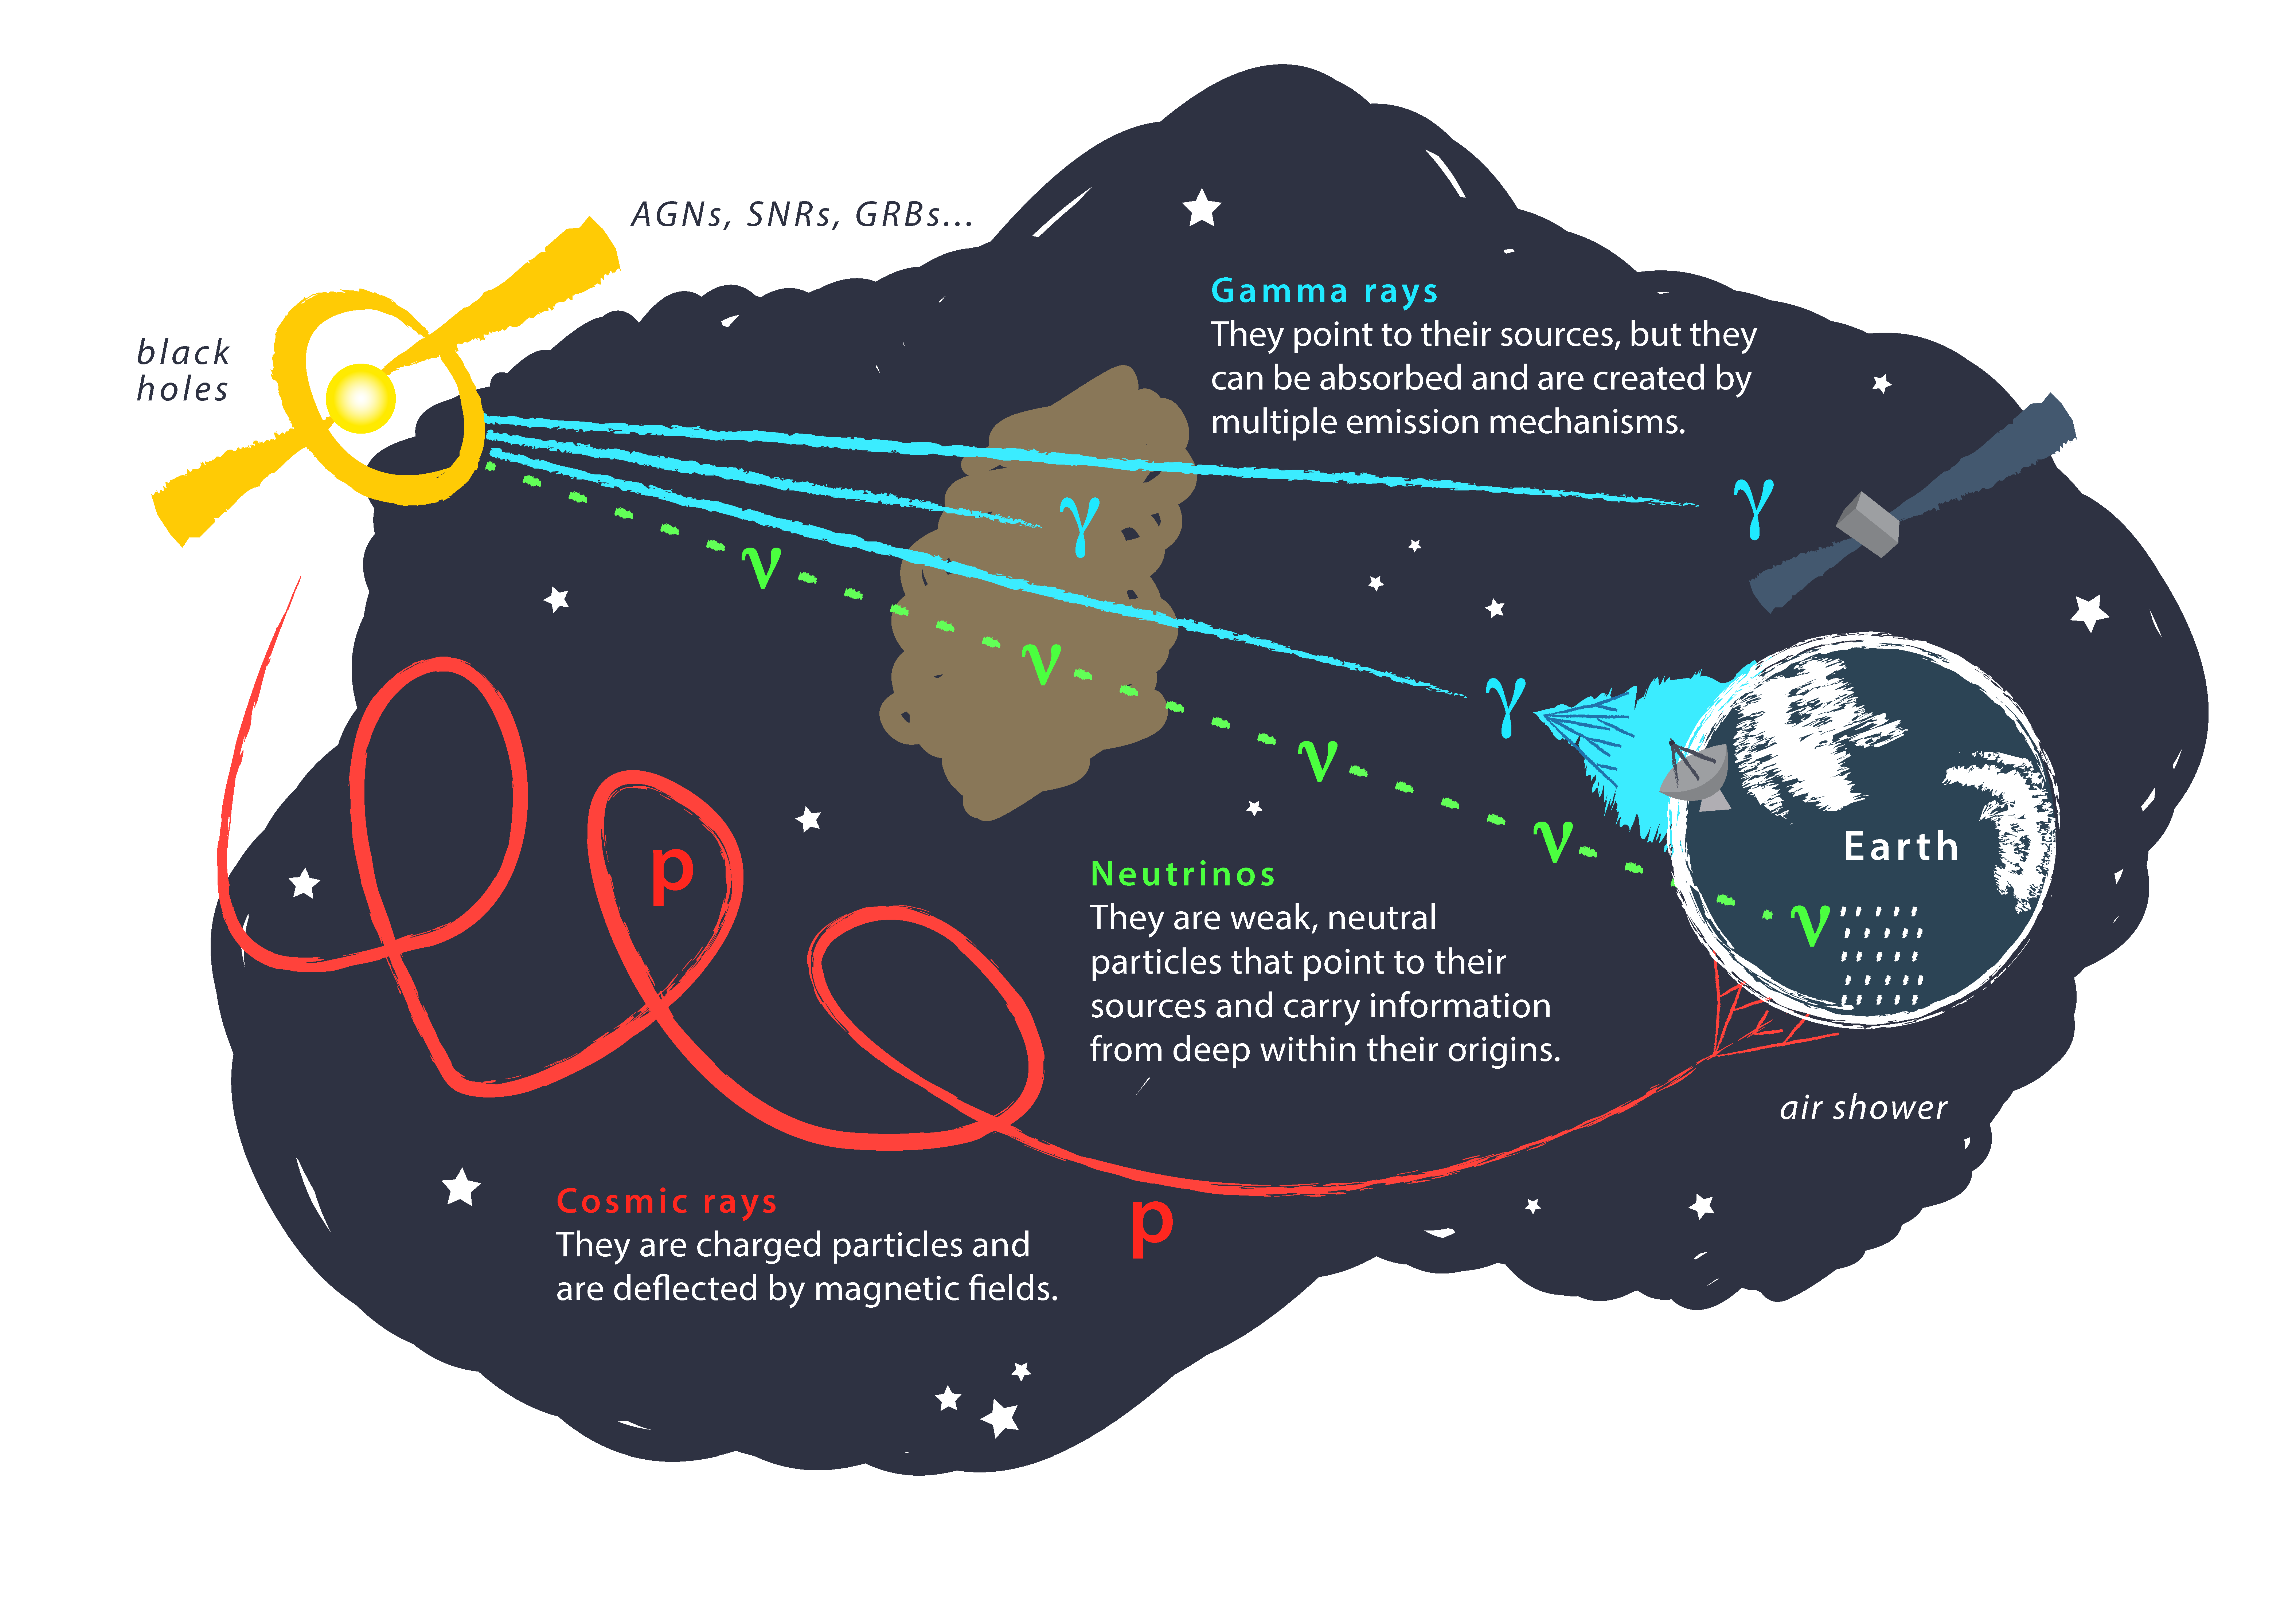
\includegraphics[width=0.9\textwidth]{images/cosmic_messengers.png}
    \caption{Only uncharged particles carry information about their origin when they arrive on earth.
        Neutrinos are hard to detect as they only interact via the weak force.
        Photons on the other hand can be absorbed in gas clouds, but are detectable using satellite- and ground-based observeratories.
    }
    \label{fig:mma}
\end{figure}

Photons and neutrions are of special interest as they are not influenced by cosmic electromagentic fields and therefore it is possible to reconstructed their origin 
position and study their sources.
As high energy gamma radiation cannot be produced thermally, more complex processes involving charged particles (Cosmic Rays) have to be considered 
(Further information in \cite{s_funk}).

The most important source class within our own galaxy are supernova remnants like the Crab Nebula \cite{nuimeprn12618}. 
Because of its constantly high gamma ray flux the Crab Nebula is often used as a "standart candle" in Gamma Ray Astronomy, observations of which are also 
analysed as part of this work.
Extragalactic sources for gamma rays are mostly supermassive black holes at the center of very bright galaxies, so called active galactic nuclei (AGN).
These black holes accrete matter from its surroundings resulting in the formation of disks around the black holes and sometimes relativistic jets are emitted 
perpendicular to the disk.
AGNs are classified depending on if a jet is emitted, how bright they are and at which angle they are observed as shown in \autoref{fig:agn}.
One of closest to earth examples of a blazar is Markarian 421 located at a redshift of $z = \num{0.03}$ \cite{Albert_2007} and observations of it are analysed in 
\autoref{ch:results}.
\begin{figure}
    \centering
    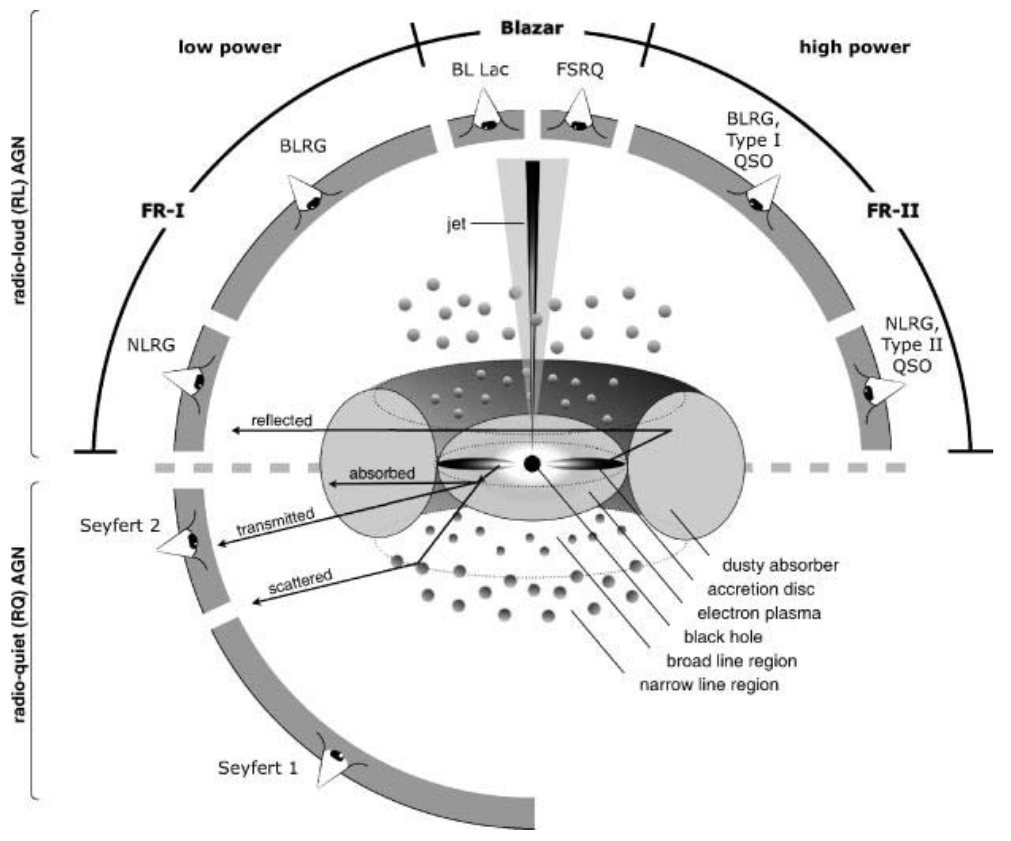
\includegraphics[width=0.8\textwidth]{images/agn.png}
    \caption{AGNs consist of a supermassive black hole in the center surrounded by an accretion disc which is again surrounded by a gas torus.
        The calssification of AGNs is based on three main characteristics, the existence of a jet, their brightness and the angle under which they can be observed \cite{doi:10.1002/9783527666829.ch4}.
    }
    \label{fig:agn}
\end{figure}


As earth's atmosphere is not transparent for high energy gamma rays, direct observations of gamma rays can only be done by satellite based observeratories 
like the Large Area Telescope on the \textit{Fermi} Gamma-Ray Space Telescope (\textit{Fermi}-LAT).
On the ground indirect observations are possible by using Imaging Air Cherenkov Telescopes (IACTs) which will be explained further in \autoref{ch:cta}.


\AtBeginSection{
  \begin{frame}{Overview}
    \tableofcontents[currentsection]
  \end{frame}
}

\section{CTA and the LST-1 prototype}
\chapter{Imaging Air Cherenkov Telescopes and the Cherenkov Telescope Array}
\label{ch:cta}

\section{Imaging Air Cherenkov Telescopes}
For IACTs the atmosphere itself acts as the detector medium. 
If a high energy primary particle interacts with the atmosphere it starts a cascade of secondary paricles called air showers.
The charged secondary particles travel faster than the speed of light in air resulting in the emission of Cherenkov Light.
This light is emitted along the moving direction of the charged particle.
The Cherenkov Light is then collected by mirrors and projected onto a camera system which is able to record single photons with a time resolution of a few nanoseconds.

As both charged primary paricles and photons start air showers a dominant background of hadronic air showers is recorded by IACTs.
In hadronic air showers many different interactions are possible due to the strong force.
These varied interactions lead to the more complex shower pattern of hadronic air showers resulting in the possibility to distinguish them from purely electromagnetic
air showers caused by photons or electrons.
Electromagnetic air showers only consist of two processes. 
High energy photons produce electron-positron pairs and the total energy of those two paricles equals the photon energy. 
High energy electrons/positrons then generate photons again through bremsstahlung. 
These two processes continue until the photon energy falls under energy threshold for pair production of $\SI{1022}{\kilo\electronvolt}$.


\section{CTA and the LST-1 prototype}
The Cherenkov Telescope Array (CTA) aims to be the next generation IACT experiment by providing a sensitivity at least an order of magnitude better than current experiments.
It will be comprised of two sites, one in the northern and one in the southern hemisphere which will consist of differently sized telescopes. 
The smallest one will be the Small-Sized Telescope (SST) sensitive for the highest energies above $\SI{5}{\tera\electronvolt}$ up until $\SI{300}{\tera\electronvolt}$.
The Medium-Sized Telescope (MST) is most sensitive for energies between $\SI{150}{\giga\electronvolt}$ and $\SI{5}{\tera\electronvolt}$ and the 
Large-Sized Telescope (LST) will cover the lowest energies from $\SI{20}{\giga\electronvolt}$ up until $\SI{150}{\giga\electronvolt}$.
A size comparsion of the telescopes can be seen in \autoref{fig:telescopes}.
\begin{figure}
    \centering
    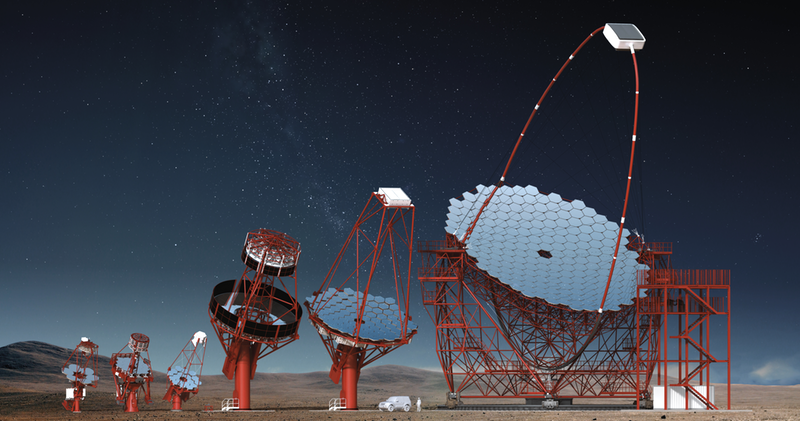
\includegraphics[width=0.8\textwidth]{images/CTA_telescopes.png}
    \caption{A depiction of the different telescopes that will be used to build CTA. 
        Three prototypes are currently being tested for the SST, two for the MST and one for the LST \cite{cta-website}.
    }
    \label{fig:telescopes}
\end{figure}

The southern site will be located in the Atacama desert in Chile and will consist of \num{4} LSTs, \num{25} MSTs and \num{70} SSTs.
The northern site will be build as part of the Observatorio del Roque de los Muchachos (ORM) on LaPalma and will include \num{4} LSTs and \num{15} MSTs.
More information about the CTA and its scientific capabilities can be found in \cite{science_with_cta}.

***More info about the sites/SST, MST ?***

The ORM is also the location of the first prototype for the LSTs inaugurated on the 10 October 2018, the LST-1 which is the subject of this work \cite{lst_inauguration}.
The LST-1 has a parabolic mirror with a diameter of $\SI{23}{\meter}$ which helps to collect the Cherenkov light of the dimmest low-energy air showers.
The light is recorded by a $\num{1855}$-pixel camera based on photomultiplier tubes with a field of view of about $\SI{4.3}{\degree}$ \cite{cta-website}.



\section{Data used and preprocessing}
\chapter{Preprocessing of the data}
\label{ch:prepro}

Before the analysis steps done in this work can be performed, the raw data taken by the LST-1 has to be processed up until what is called Data Level 1 (DL1).
For this work such preprocessing was done using \texttt{lstchain}, a low-level data processing pipeline for the LST telescopes. 
\texttt{lstchain} is open-source project which is still in development on github \cite{lstchain} and is based on \texttt{ctapipe}. 
\texttt{ctapipe} will be the main low-level data processing pipeline for CTA and is itself in development as an open-source project.
This work uses the versions \texttt{v0.5.1} and \texttt{v0.5.2} of \texttt{lstchain} which are both based on version \texttt{v0.7.0} of \texttt{ctapipe} \cite{ctapipe}. 

In the first step the waveforms recorded by each pixel of the camera are cleaned to reduce the influence of electronic noise in the signal.
After that the waveforms are integrated to obtain the total photon charge and a mean arrival time for the photons is defined for each pixel 
as the point in time at which half of all the photons within the pixel have arrived.
This results in two 2-dimensional images for each event recorded by the camera, as can be seen in \autoref{fig:eas_images}.
\begin{figure}
    \centering
    \begin{subfigure}{0.49\textwidth}
        \centering
        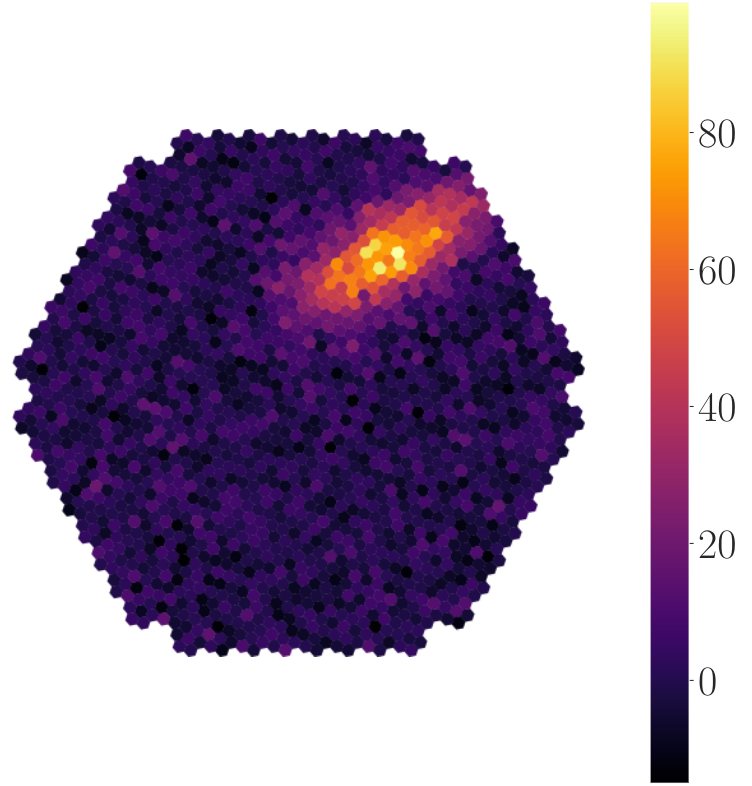
\includegraphics[width=0.8\textwidth]{images/eas_image1.png}
        \caption{Number of photons per pixel.}
        \label{fig:eas_image1}
    \end{subfigure}
    \hfill
    \begin{subfigure}{0.49\textwidth}
        \centering
        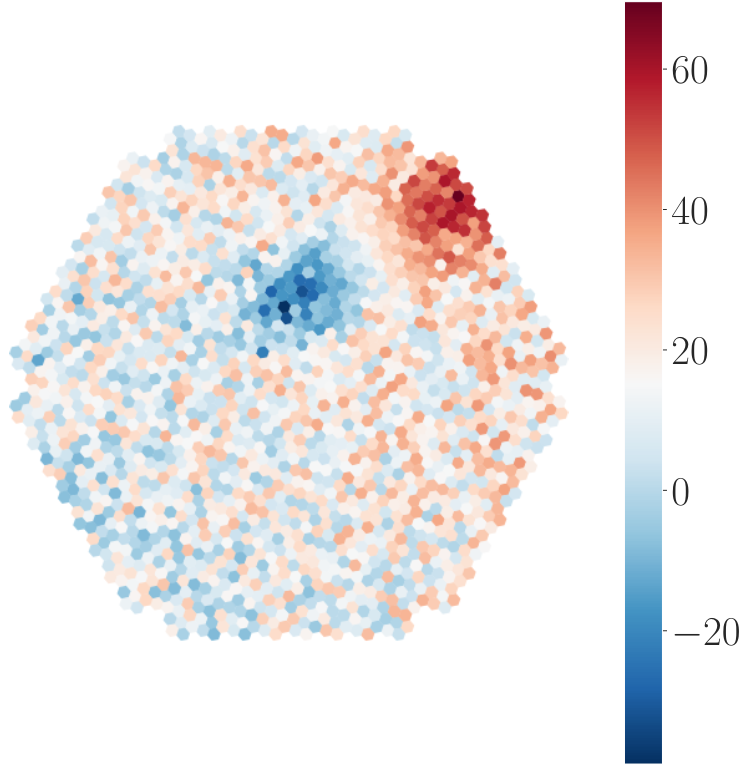
\includegraphics[width=0.8\textwidth]{images/eas_image2.png}
        \caption{Arrival time per pixel relative to the mean arrival time for the whole image.}
        \label{fig:eas_image2}
    \end{subfigure}
    \caption{The integrated photon count in \subref{fig:eas_image1} showes the air shower clearly but a lot of noise is visible in the non-shower pixels.
        The arrival times in \subref{fig:eas_image2} show a clear correlation for the pixels that recorded the air shower \cite{lukas}.
    }
    \label{fig:eas_images}
\end{figure}

In the next step these images are cleaned by discarding pixels that did not record the air shower. 
This is done in multiple steps using two thresholds for the photon charge of each pixel and one for the number of neighboring pixels.
First all pixels above the higher photon charge threshold with enough neighboring pixels above the lower photon charge threshold get selected as part of the shower.
After that all pixels above the lower photon charge threshold with enough neighboring pixels above the higher photon charge threshold get selected as well \cite{lukas}.
For rather soft thresholds the results of this cleaning can be seen in \autoref{fig:eas_images_cleaned}.
\begin{figure}
    \centering
    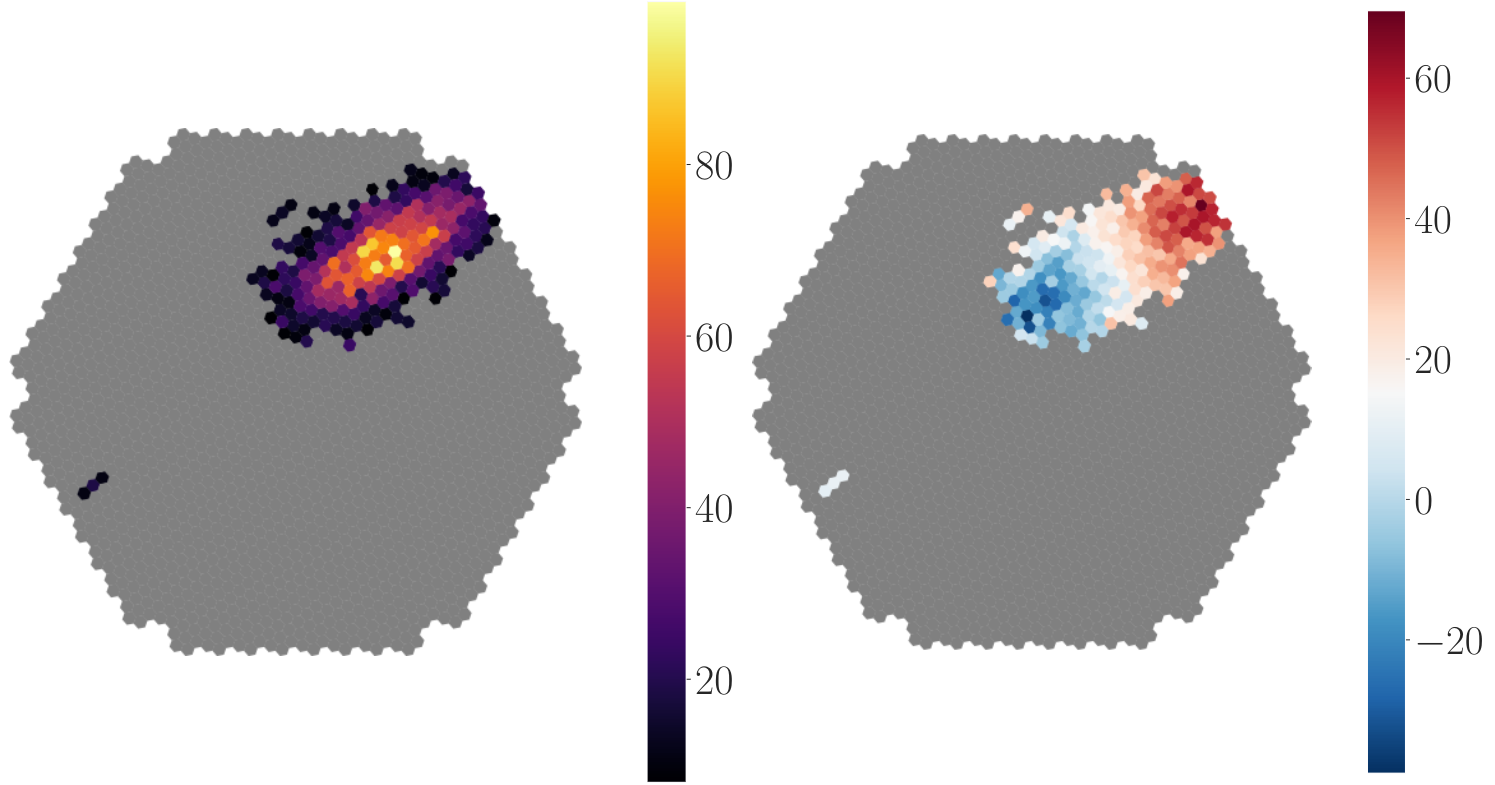
\includegraphics[width=0.8\textwidth]{images/eas_images_cleaned.png}
    \caption{The pixels discarded during the image cleaning are marked as grey. The soft thresholds chosen for this example result in two smaller pixel-islands remaining \cite{lukas}.}
    \label{fig:eas_images_cleaned}
\end{figure}

Based on these cleaned images, a multitude of image parameters can be calculated.
The most important ones are the total number of photons in the shower, \texttt{intensity}, and the so called hillas parameters which are illustrated in \autoref{fig:image_parameters}.
the hillas parameters are based on a principal component analysis (PCA) of the photon charge distribution and describe the extension and orientation of the shower.
The parameters \texttt{length} and \texttt{width} correspond with the standard deviations along the principal components of the distribution and are therefore a 
description of the shower extension. 
The orientation on the other hand is described by the angle of the main shower axis relative to the $x$-axis of the image.
The performance of the algorithms used in this work in regards to reconstructing this angle can be seen in \autoref{fig:delta_comparison}.
\begin{figure}
    \centering
    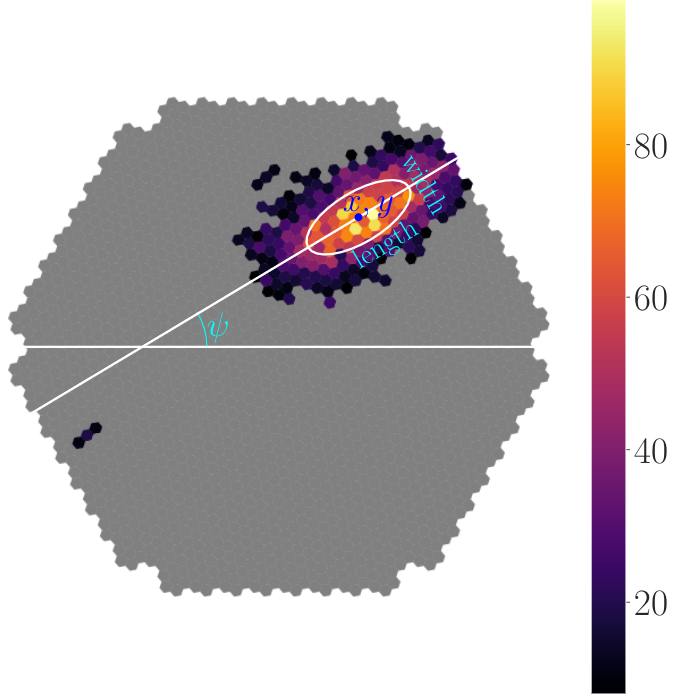
\includegraphics[width=0.5\textwidth]{images/image_parameters.png}
    \caption{The PCA-based hillas-parameters calculated for the cleaned image of the integrated photon count.
        $\Psi$ describes the angle of the main shower axis relative to the x-axis of the image and $x$ and $y$ are the coordinates of the center of gravity of the shower. 
        \texttt{length} and \texttt{width} can be depicted as the semi-major and semi-minor axis of an ellipse \cite{lukas}.
    }
    \label{fig:image_parameters}
\end{figure}

Higher moments of the distribution like \texttt{skewness} and \texttt{kurtosis} are also calculated. 
The center of gravity of the shower image is calculated by weighting the coordinates of each pixel with the photon charge of this pixel.
Additional image featueres include multiple \texttt{leakage} parameters that describe how much of the light was recorded at the edge of the camera and are
therefore an indication of how much light from the shower might have missed the camera.

The image of the arrival times allows for timing parameters to be calculated by fitting a linear function along the main shower axis. 
This yields the parameters \texttt{time\_gradient} and \texttt{intercept} which help to determine the direction of the shower, together with \texttt{skewness}.

\section{Reconstruction of physical properties using machine learning}
\begin{frame}{Event pre-selection}
    \begin{columns}[onlytextwidth, t]
        \begin{column}{0.45\textwidth}
            \begin{align*}
                \mathtt{intensity} &> 300\\
                \mathtt{leakage1\_intensity} &< 0.2\\
                \mathtt{leakage2\_intensity} &< 0.2
            \end{align*}
            \begin{itemize}
                \item[\textbf{\textcolor{green}{+}}] Remove incomplete shower images
                \item[\textbf{\textcolor{green}{+}}] Remove dim events
                \item[\textbf{\textcolor{red}{-}}] Remove low energy events
            \end{itemize}
        \end{column}
        \begin{column}{0.45\textwidth}
            \only<2>{
                \begin{align*}
                    \mathtt{intensity} &> 150\\
                    \mathtt{leakage1\_intensity} &< 0.2\\
                    \mathtt{leakage2\_intensity} &< 0.2
                \end{align*}
                \begin{itemize}
                    \item[\textbf{\textcolor{green}{+}}] Lower energy events included
                    \item[\textbf{\textcolor{red}{-}}] which are harder to reconstruct
                \end{itemize}
            }
        \end{column}
    \end{columns}

    \note<1->[item]{Zuerst Eventselektion $\to$ diese Kriterien}
    \note<1->[item]{\texttt{leakage} $\to$ entferne unvollständige Bilder}
    \note<1->[item]{\texttt{intensity} $\to$ entferne dunkle Bilder (hell besser rekonstruierbar)}
    \note<2->[item]{Derart großer Wert für \texttt{intensity} $\to$ entfernt niederenergetische Ereignisse
        \newline $\to$ Wert verringern \newline
    }
    \note<2->[item]{Plots im Folgenden: v0.5.2 + \texttt{intensity > 300}}
\end{frame}

\begin{frame}{The aict-tools}
    \begin{columns}[onlytextwidth]
        \begin{column}{0.65\textwidth}
            \begin{itemize}
                \item Apply event pre-selection
                \item Train and apply scikit-learn models for 
                    \begin{itemize}
                        \item Gamma-hadron separation
                        \item Energy estimation
                        \item Origin reconstruction
                    \end{itemize}
                \item Create performance plots
            \end{itemize}
            \medskip
            \onslide<2->{
                Commandline applications \& configuration using a single YAML-file
                \begin{itemize}
                    \item[\textbf{\textcolor{tugreen}{\to}}] automated pipeline using make \textbf{\textcolor{tugreen}{\to}} reproducibility
                \end{itemize}
                Initially developed for FACT 
                \begin{itemize}
                    \item Different conventions than CTA (e.g. camera frame definition, units)
                        \begin{itemize}
                            \item[\textbf{\textcolor{tugreen}{\to}}] Conversion of LST data necessary
                        \end{itemize}
                    \item Continued development adds more CTA support 
                        \begin{itemize}
                            \item[\textbf{\textcolor{tugreen}{\to}}] Only data-structure adjustment and some renaming necessary now
                        \end{itemize}
                \end{itemize}
            }
        \end{column}
        \begin{column}{0.33\textwidth}
            \centering
            
\includegraphics[width=\textwidth]{images/python.png}
            
\includegraphics[width=0.8\textwidth]{images/scikit.png}
            
\includegraphics[width=\textwidth]{images/pandas.png}
        \end{column}
    \end{columns}
    \onslide<2->{
        \begin{center}
            \vspace{0.5\baselineskip}
            \small\fullcite{aict-tools}
        \end{center}
    }

    \note<1->[item]{Durchführung der Analyse: aict-tools}
    \note<1->[item]{- Eventselektion anwenden
        \newline - Modelle des ML trainieren \& anwenden 
        \newline - scikit-learn Modelle 
        \newline - für Teilchentypbestimmung, Energieschätzung und Richtungsrekonstruktion
        \newline - Performance plots
    }
    \note<2->[item]{Vorteil: Anwendung mit Kommandozeile \& Konfiguration mit 1 YAML-Datei
        \newline $\to$ Analyse automatisieren 
        \newline $\to$ Reproduzierbarkeit 
        \newline $\to$ + Hier: Vergleich Kombinationen
    }
    \note<2->[item]{Ursprünglich für FACT entwickelt 
        \newline $\to$ Andere Konventionen 
        \newline $\to$ LST Daten anpassen
        \newline $\to$ Während Arbeit: Weiterentwicklung 
        \newline $\to$ nur noch minimale Anpassungen nötig
    }
\end{frame}

\begin{frame}{The disp method}
    \begin{columns}[onlytextwidth]
        \begin{column}{0.475\textwidth}
            \begin{itemize}
                \setlength\itemsep{1em}
                \item Origin reconstruction is 2D regression task 
                \item Assuming the main shower axis is correctly reconstructed\\
                    \begin{itemize}
                        \item[\textbf{\textcolor{tugreen}{\to}}] Estimate distance along axis $\to$ 1D regession
                        \item[\textbf{\textcolor{tugreen}{\to}}] Decide which side of cog $\to$ classification
                    \end{itemize}
            \end{itemize}
        \end{column}
        \begin{column}{0.475\textwidth}
            \centering
            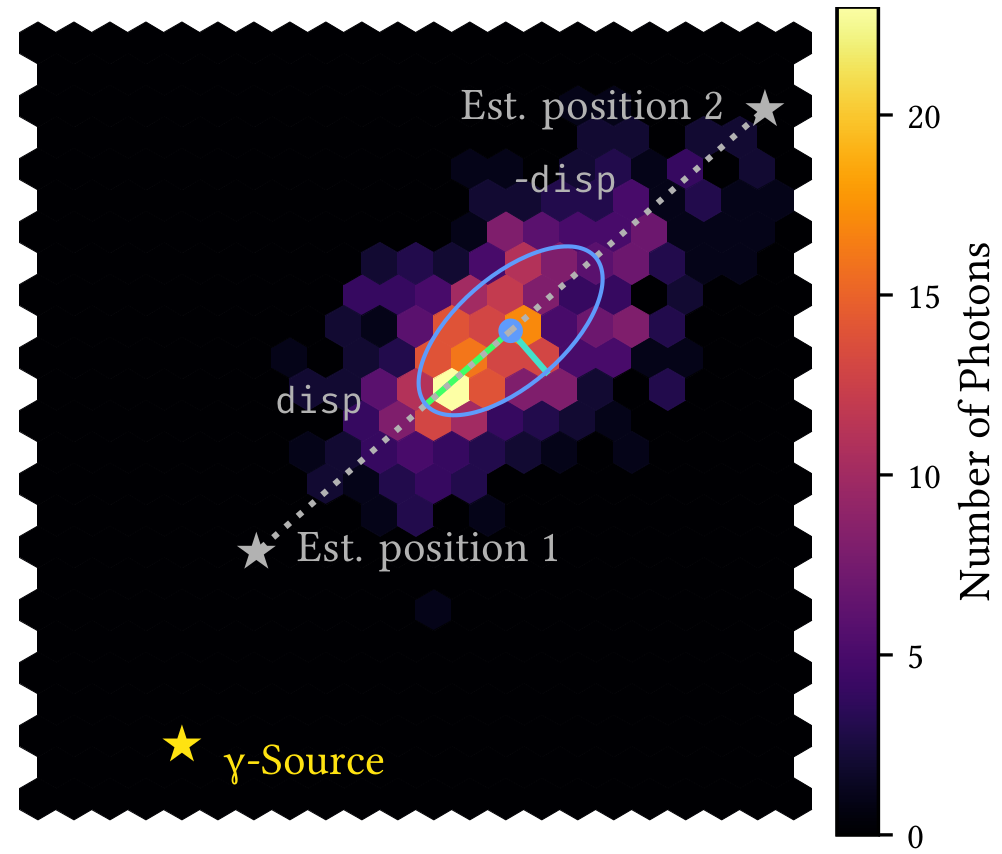
\includegraphics[width=\textwidth]{images/disp.png}\\[-0.5\baselineskip]
            \hspace{1.5cm}\href{https://github.com/MaxNoe/phd_thesis}{[Max Noethe, PhD thesis]}
        \end{column}
    \end{columns}

    \note[item]{Richtungsrekonstruktion aict-tools $\to$ disp Methode}
    \note[item]{Normalerweise 2D Regression}
    \note[item]{Annahme: Hauptachse korrekt rekonstruiert
        \newline $\to$ Abstand Quelle entlang Hauptachse
        \newline $\to$ + Entscheidung welche Seite von Schwerpunkt
    }
\end{frame}

\section{Model performance}
\begin{frame}{Gamma-hadron separation}
    \begin{columns}[onlytextwidth]
        \begin{column}{0.475\textwidth}
            \centering
            \includegraphics[width=\textwidth]{../HDD/build_scaling_300/plots_separator/plot_4.pdf}
        \end{column}
        \begin{column}{0.475\textwidth}
            \begin{itemize}
                \setlength\itemsep{1em}
                \item Random forest classifier
                    \begin{itemize}
                        \item Trained on diffuse gammas and protons
                        \item \texttt{gamma\_prediction} score $\in [0, 1]$
                        \item[\textbf{\textcolor{tugreen}{\to}}] Choose prediction threshold $t_\gamma$
                    \end{itemize}
                \item Differentiate gamma-hadron shower images
                    \begin{itemize}
                        \item[\textbf{\textcolor{tugreen}{\to}}] Features describing shower image are most important
                    \end{itemize}
            \end{itemize}
        \end{column}
    \end{columns}

    \note[item]{Teilchentypbestimmung 
        \newline $\to$ Random forest Algo. zur Klassifizierung
        \newline $\to$ Trainiert: diffuse Gammas und Protonen
        \newline $\to$ Jedes Ereignis: \texttt{gamma\_prediction} Wert 
        \newline $\to$ Schwellwert für \texttt{gamma\_prediction}
    }
    \note[item]{Entscheidungsbaum basierter Algo. $\to$ Wichtigkeit Bildparameter}
    \note[item]{Komplexe hadronische Schauer $\to$ komplexere Bilder 
        \newline $\to$ Bildparameter für Schauerform
    }
\end{frame}

\begin{frame}{Gamma-hadron separation}
    \begin{columns}[onlytextwidth]
        \begin{column}{0.5\textwidth}
            \centering
            \includegraphics[width=1.1\textwidth]{../HDD/build_scaling_300/plots_separator/plot_1.pdf}
        \end{column}
        \begin{column}{0.5\textwidth}
            \begin{itemize}
                \item Perfromance evaluation independent from prediction threshold $t_\gamma$
            \end{itemize}
            \begin{table}
                \caption{Mean area under ROC Curve.}
                \sisetup{table-format=0.3}
                \begin{tabular}{ S  S  S}
                    \toprule
                     & {lstchain v0.5.1} & {lstchain v0.5.2} \\
                    \midrule
                    \texttt{intensity > 300} & 0.907 & 0.944 \\
                    \texttt{intensity > 150} & 0.860 & 0.908 \\
                    \bottomrule
                \end{tabular}
            \end{table}
        \end{column}
    \end{columns}

    \note[item]{Perfromance Klassifizier unabhängig Wahl Schwellwert 
        \newline $\to$ Fläche unter ROC Kurve $\to$ Bild
    }
    \note[item]{Ergebnisse verschiedene Kombinationen $\to$ Tabelle
        \newline $\to$ v0.5.2 deutlich besser
    }
\end{frame}

%%%%%%%%%%%%%%%%%%%%%%%%%%%%%%%%%%%%%%%%%%%%%%%%%%%%%%%%%%%%%%%%%%%%%%%%%%%%%%%%%%%%%%%%%%%%%%%%%%%%%%%%%%%%
\begin{frame}{Energy estimation}
    \begin{columns}[onlytextwidth]
        \begin{column}{0.475\textwidth}
            \centering
            \includegraphics<1>[width=\textwidth]{../HDD/build_scaling_300/plots_regressor/plot_4.pdf}
            \includegraphics<2>[width=\textwidth]{../HDD/build_scaling_300/plots_regressor/plot_1.pdf}
        \end{column}
        \begin{column}{0.475\textwidth}
            \begin{itemize}
                \setlength\itemsep{1em}
                \item Random forest regressor
                \item Trained on point-like gammas
                \item Light content most important
            \end{itemize}
        \end{column}
    \end{columns}

    \note<1->[item]{Energieschätzung 
        \newline $\to$ Random Forest
        \newline $\to$ Trainiert: Punktquellen Gammas    
    }
    \note<1->[item]{Beitrag Bildparameter $\to$ Helligkeit beschriebende Parameter}
    \note<2->[item]{Mögleichkeit Performance Regressor darzustellen $\to$ Migrations Matrix}
\end{frame}

\begin{frame}{Energy estimation}
    \begin{columns}[onlytextwidth]
        \begin{column}{0.5\textwidth}
            \centering
            Bias
            \includegraphics[width=\textwidth]{build/plot_talk_2.pdf}
        \end{column}
        \begin{column}{0.5\textwidth}
            \centering
            (Quantile) Resolution
            \includegraphics[width=\textwidth]{build/plot_talk_3.pdf}
        \end{column}
    \end{columns}

    \note[item]{Verrzerrung für verschiedene Kombinationen:
        \newline $\to$ Niedrige E: Überschätzt, da nur helle Ereignisse
        \newline $\to$ Hohe E: Unterschätzt, da Schauer nicht ganz im Kamera
    }
    \note[item]{Auflösung: 
        \newline $\to$ Insgesamt besser für höhere Energien
    }
    \note[item]{\texttt{intensity > 300} Kombinationen schlechter bei niedrige E $\to$ wenige, helle Ereignisse}
\end{frame}

%%%%%%%%%%%%%%%%%%%%%%%%%%%%%%%%%%%%%%%%%%%%%%%%%%%%%%%%%%%%%%%%%%%%%%%%%%%%%%%%%%%%%%%%%%%%%%%%%%%%%%%%%%%%
\begin{frame}{Origin reconstruction}
    \begin{columns}[onlytextwidth]
        \begin{column}{0.475\textwidth}
            \begin{itemize}
                \setlength\itemsep{1em}
                \item Random forest regressor/ classifier
                \item Trained on diffuse gammas
                \item Timing parameters and skewness (3rd moment along main shower axis) very important
            \end{itemize}
        \end{column}
        \begin{column}{0.475\textwidth}
            \centering
            \includegraphics<1>[width=\textwidth]{../HDD/build_scaling_300/plots_disp/plot_6.pdf}
            \includegraphics<2>[width=\textwidth]{../HDD/build_scaling_300/plots_disp/plot_5.pdf}
        \end{column}
    \end{columns}

    \note[item]{Richtungsrekonstruktion: disp \& sign
        \newline $\to$ erneut Random Forest
        \newline $\to$ Trainiert: Diffuse Gammas 
    }
    \note[item]{Parameter anhand Ankunftszeiten und Schiefe (entlang Hauptachse) wichtig}
    \note<2->[item]{$\to$ besonders bei sign}
\end{frame}

\begin{frame}{Origin reconstruction: angular resolution}
    \begin{columns}[onlytextwidth]
        \begin{column}{0.5\textwidth}
            \centering
            v0.5.2 and intensity > 300
            \includegraphics[width=\textwidth]{../HDD/build_scaling_300/plots_crab/plot_9.pdf}
        \end{column}
        \begin{column}{0.5\textwidth}
            \centering
            correct sign and $p_\gamma > 0.6$
            \includegraphics[width=\textwidth]{build/plot_talk_1.pdf}
        \end{column}
    \end{columns}

    \note[item]{Insgesamt Performance Richtungsrekonstruktion $\to$ Winkelauflösung
        \newline $\to$ Radius in dem 68\% der Ereignisse einer Punktquelle rekonstruiert
    }
    \note[item]{Sinnvolle Einschränkung 
        \newline $\to$ Nur events mit korrektem sign $\to$ sonst weit weg von echter Quelle
        \newline $\to$ + Ereignisse, die wahrsch. Gammas
    }
    \note[item]{Vergleich Kombinationen 
        \newline $\to$ deutliche Verbesserung mit v0.5.2
        \newline $\to$ \texttt{intensity > 300} besser als \texttt{intensity > 150}
    }
\end{frame}

\section{Results for observational data}
\begin{frame}{Detection of the Crab Nebula}
    \begin{columns}[onlytextwidth]
        \begin{column}{0.64\textwidth}
            \centering
            \includegraphics[width=\textwidth]{../HDD/build_scaling_300/plots_crab/plot_2.pdf}
        \end{column}
        \begin{column}{0.35\textwidth}
            \hspace{0.3cm}\textcolor{tugreen}{Date:} 18th January, 2020\\
            \hspace{0.3cm}\textcolor{tugreen}{ON:} \SI{2.6}{\hour}\\
            \hspace{0.3cm}\textcolor{tugreen}{OFF:} \SI{1.3}{\hour}\\
            \medskip
            \begin{itemize}
                \item Different observation times for ON and OFF $\to$ scaling necessary:
                    \begin{align*}
                        \alpha = \frac{N_\text{on}(\SI{0.5}{\degree\squared} < \theta^2 < \SI{1}{\degree\squared})}
                            {N_\text{off}(\SI{0.5}{\degree\squared} < \theta^2 < \SI{1}{\degree\squared})}
                    \end{align*}
                \item $\theta^2_\text{max}$ and $t_\gamma$ optimised for maximum detection significance
            \end{itemize}
        \end{column}
    \end{columns}

    \note[item]{Krebsnebel}
    \note[item]{Unterschieliche Beobachtungszeit $\to$ Ereignisraten skalieren
        \newline Alle Ereignisse $\SI{0.5}{\degree\squared} < \theta^2 < \SI{1}{\degree\squared}$ vergleichen
    }
    \note[item]{Radius $\theta^2_\text{max}$ \& Schwellwert $t_\gamma$ für Berechung festlegen $\to$ Detektionssignifikanz
        \newline $\to$ Signifikans von 27.7$\sigma$ 
        \newline $\to$ $\theta^2_\text{max}$ und $t_\gamma$ hier optimiert
    }
\end{frame}

\begin{frame}{Detection of Markarian 421}
    \begin{columns}[onlytextwidth]
        \begin{column}{0.64\textwidth}
            \centering
            \includegraphics[width=\textwidth]{../HDD/build_scaling_300/plots_mrk421/plot_2.pdf}
        \end{column}
        \begin{column}{0.35\textwidth}
            \hspace{0.3cm}\textcolor{tugreen}{Date:} 20th June, 2020\\
            \hspace{0.3cm}\textcolor{tugreen}{Wobble:} \SI{2.2}{\hour}\\
            \medskip
            \begin{itemize}
                \item $n = \num{5}$ OFF regions
            \end{itemize}
        \end{column}
    \end{columns}

    \note[item]{Wobble Mode von Markarian 421}
    \note[item]{n = 5 äquidistante OFF regionen entlang Kreis}
    \note[item]{$\theta^2_\text{max}$ und $t_\gamma$ wie Krebsnebel $\to$ Signifikanz von 43.7$\sigma$ erreicht}
\end{frame}

\section{Conclusion and Outlook}
\begin{frame}[t]{Conclusion and Outlook}
    \begin{columns}[onlytextwidth]
        \begin{column}[T]{0.43\textwidth}
            \begin{itemize}
                \setlength\itemsep{1em} %!!!!!!!!!!!!!!!!!!!!!!!!!!!!!!!!
                \item<1-> aict-tools achieve good results for high energies
                \item<1-> lstchain v0.5.2 improved results
                    \begin{itemize}
                        \item[\textbf{\textcolor{tugreen}{\to}}] Impact of other changes besides scaling of optical efficiency?
                    \end{itemize}
                \item<2-> Optimisation of event pre-selection
                \item<2-> Energy dependent $\theta^2_\text{max}$ and $t_\gamma$ cuts optimised on simulations
                \item<2-> Wobble mode observations of the Crab Nebula
            \end{itemize}
        \end{column}
        \begin{column}[T]{0.55\textwidth}
            \vspace{-1cm}
            \begin{tikzpicture}
                \roundpic[xshift=0cm,yshift=0cm]{7.8cm}{14cm}{images/LST_1.jpg}{2}{1.5}
                \node[circle, fill, color=white, minimum width = 4.2cm] at (-3.6,3.3){};
                \roundpic[xshift=-.2cm,yshift=-.2cm]{4.2cm}{4.25cm}{../build/plot_talk_1.pdf}{-3.6}{3.3}
                \node[circle, fill, color=white, minimum width = 4.9cm] at (-1,0){};
                \roundpic[xshift=-.2cm,yshift=-.2cm]{4.9cm}{4.95cm}{../HDD/build_scaling_300/plots_crab/plot_2.pdf}{-1}{0}
            \end{tikzpicture}
        \end{column}
    \end{columns}

    \note[item]{Gute Ergebnisse für LST-1 mit aict-tools möglich}
    \note[item]{Verbesserung mit lstchain v0.5.2
        \newline $\to$ Andere Änderungen vgl. mit v0.5.1?
    }
    \note<2->[item]{Nur 3 Parameter für Eventselektion $\to$ Optimierbar!}
    \note<2->[item]{$\theta^2_\text{max}$ Radius und $t_\gamma$ Schwellwert besser auf Simulation optimieren!}
    \note<2->[item]{Krebsnebeldaten alt $\to$ neue (wobble!) Daten vermutlich besser!}
\end{frame}


\begin{frame}
  \centering 
  \Huge\color{tugreen} Backup
\end{frame}

\begin{frame}{Accuracy sign \& $r^2$-score |disp|}
    \begin{columns}[onlytextwidth]
        \begin{column}{0.49\textwidth}
            \centering
            \small v0.5.2 and intensity > 300\\
            \includegraphics[width=.6\textwidth]{../HDD/build_scaling_300/plots_disp/plot_8.pdf}\\
            \small v0.5.1 and intensity > 300\\
            \includegraphics[width=.6\textwidth]{../HDD/build_noscaling_300/plots_disp/plot_8.pdf} 
        \end{column}
        \begin{column}{0.49\textwidth}
            \centering
            \small v0.5.2 and intensity > 150\\
            \includegraphics[width=.6\textwidth]{../build/plots_disp/plot_8.pdf}\\
            \small v0.5.1 and intensity > 150\\
            \includegraphics[width=.6\textwidth]{../HDD/build_noscaling/plots_disp/plot_8.pdf}  
        \end{column}
    \end{columns} 
\end{frame}

\begin{frame}{Crab Nebula: v0.5.2 and intensity > 300}
    \begin{columns}[onlytextwidth]
        \begin{column}{0.65\textwidth}
            \centering
            \includegraphics[width=\textwidth]{../HDD/build_scaling_300/plots_crab/plot_1.pdf}
        \end{column}
        \begin{column}{0.3\textwidth}
            \begin{itemize}
                \item $\alpha = \frac{t_\text{on}}{t_\text{off}}$
            \end{itemize}   
        \end{column}
    \end{columns}  
\end{frame}

\begin{frame}{Crab Nebula: v0.5.2 and intensity > 150}
    \centering
    \includegraphics[width=0.65\textwidth]{../build/plots_crab/plot_2.pdf}
\end{frame}

\begin{frame}{Crab Nebula: v0.5.1 and intensity > 300}
    \centering
    \includegraphics[width=0.65\textwidth]{../HDD/build_noscaling_300/plots_crab/plot_2.pdf}
\end{frame}

\begin{frame}{Crab Nebula: v0.5.1 and intensity > 150}
    \centering
    \includegraphics[width=0.65\textwidth]{../HDD/build_noscaling/plots_crab/plot_2.pdf}
\end{frame}

\end{document}
